\documentclass[letterpaper,12pt]{article}

\usepackage[utf8]{inputenc}
\usepackage[spanish,mexico]{babel}
% Usar codificación T1
\usepackage[T1]{fontenc}

\usepackage[lmargin=2cm,rmargin=2cm,top=3cm,bottom=3cm]{geometry}

\usepackage{longtable} 
\usepackage{multirow}
\usepackage{graphicx}
\usepackage{subfigure}
\usepackage{rotating}
\usepackage{cite}

\title{Práctica 02}
\author{Jesús Esteban Sánchez Alcántara\\chuyunam93@gmail.com}
\date{\today}

\begin{document}

\maketitle


\begin{table}[h!]
\centering
\resizebox{0.8\textwidth}{!} {
\begin{tabular}{cccccccccccccc}\hline
\multicolumn{2}{|c|}{1} &\multicolumn{2}{c|}{6}& \multicolumn{2}{c|}{15} & \multicolumn{2}{c|}{20} &   \multicolumn{2}{c|}{15} & \multicolumn{2}{c|}{6} & \multicolumn{2}{c|}{1} \\ \hline 
 & \multicolumn{2}{|c|}{1} &\multicolumn{2}{c|}{5}& \multicolumn{2}{c|}{10} & \multicolumn{2}{c|}{10} &   \multicolumn{2}{c|}{5} & \multicolumn{2}{c|}{1} & \\  
 \cline{2-13}
& & \multicolumn{2}{|c|}{1} &\multicolumn{2}{c|}{4}& \multicolumn{2}{c|}{6} & \multicolumn{2}{c|}{4} &   \multicolumn{2}{c|}{1} & & \\ 
\cline{3-12}
& & & \multicolumn{2}{|c|}{1} &\multicolumn{2}{c|}{3}& \multicolumn{2}{c|}{3} & \multicolumn{2}{c|}{1} & & &\\ 
\cline{4-11}
& & & & \multicolumn{2}{|c|}{1} &\multicolumn{2}{c|}{2}& \multicolumn{2}{c|}{1} & & & &\\ 
\cline{5-10}
& & & & & \multicolumn{2}{|c|}{1} & \multicolumn{2}{c|}{1} & & & & &\\ 
\cline{6-9}
& & & & & & \multicolumn{2}{|c|}{1} & & & & & & \\ 
\cline{7-8}
\end{tabular}
}
\caption{Triángulo de Pascal invertido}
\end{table}

\newpage

\section{Medianas de un triángulo}

\begin{figure}[h!]
	\begin{minipage}{6cm}
	 	\centering
	    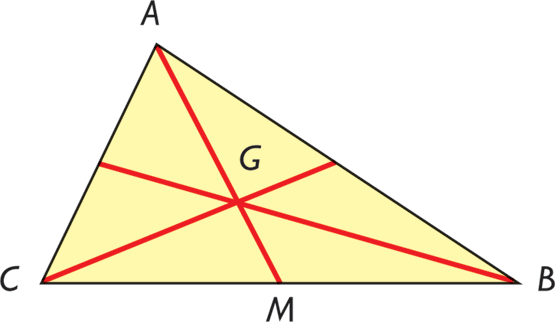
\includegraphics[scale=0.31]{medianas}
         \caption{Medianas}
    \end{minipage}
    \hspace{1.5cm}
    \begin{minipage}{10cm}
   	 En geometría las medianas de un triángulo son cada una de los tres segmentos que unen cada vértice 
	con el punto medio de su lado opuesto. Cada mediana divide al triángulo en dos regiones de igual área.
	Las tres medianas se intersecan en el baricentro, gravicentro, o centroide, marcado como G en la figura de 	la derecha. \\Vea \cite[cap. 6]{Relaciones y Geometria Analitica}
    \end{minipage}
\end{figure}

\section{Fractales}
Triángulo de Sierpinski\footnote{Todos los tríangulos corresponden a una misma imagen}. Vea \cite[2003]{Fractales y Cosas Raras}

\begin{table}[h!]
\centering
\begin{tabular}{|ccccc|}\hline
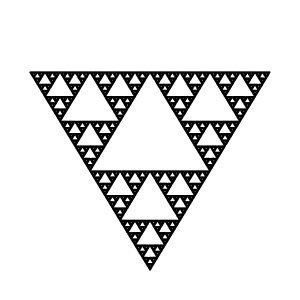
\includegraphics[scale=0.32]{fractal} &  &  &  & 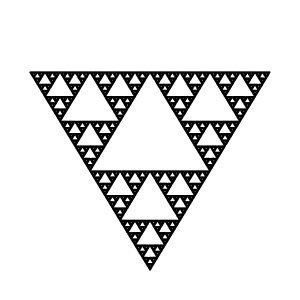
\includegraphics[scale=0.35]{fractal}\\
 & 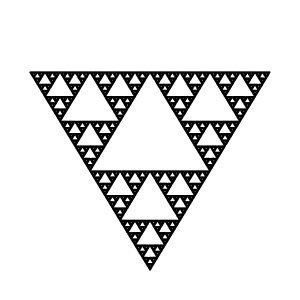
\includegraphics[angle=90,scale=0.32]{fractal} &  & 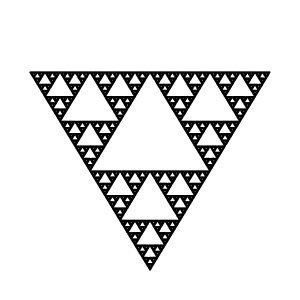
\includegraphics[angle=90,scale=0.32]{fractal} & \\
 &  & 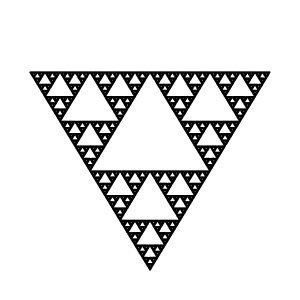
\includegraphics[angle=60,scale=0.32]{fractal} &  & \\
 & 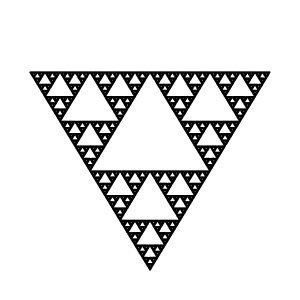
\includegraphics[angle=90,scale=0.32]{fractal} &  & 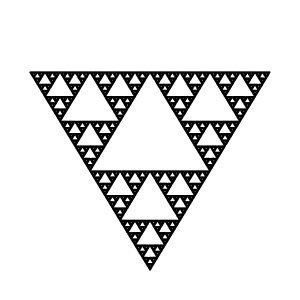
\includegraphics[angle=90,scale=0.32]{fractal} & \\
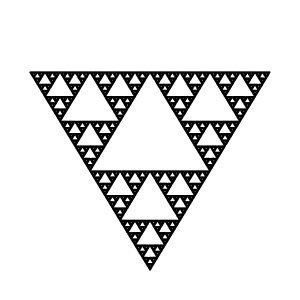
\includegraphics[angle=60,scale=0.32]{fractal} &  &  &  & 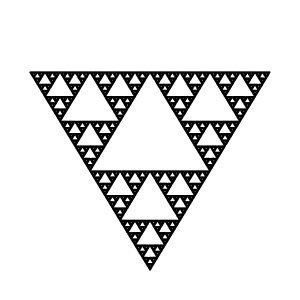
\includegraphics[angle=60,scale=0.32]{fractal}\\
\hline
\end{tabular}
\end{table}

\newpage

\section{Paquetes de \LaTeX{}}
Ejemplos de paquetes disponibles en \LaTeX{}, para más información consulte  \cite{Lamport}

\begin{table}[h!]
\centering
\begin{tabular}{|c|c|c|c|c|}
\cline{2-4}
\multicolumn{1}{c}{}& \multicolumn{3}{|c|}{\multirow{2}{*}{\textbf{Paquetes de \LaTeX{}}}}& \multicolumn{1}{c}{} \\ \cline{1-1}\cline{5-5}
\multicolumn{1}{|c}{}& \multicolumn{3}{c}{} &  \\ \hline
\textbf{Uso} & \textbf{\textit{Paquete}} & \textbf{Comandos} & \textbf{Opciones} & \textbf{IDE}\\ \hline \hline
\multicolumn{1}{|l|}{\textbf{Español y}} & \textit{babel} & \multirow{2}{*}{Ninguno} & spanish & \multirow{2}{*}{TeXLive, MikTeX}\\ 
\cline{2-2} \cline{4-4}
\multicolumn{1}{|l|}{\textbf{codificación}} & \textit{fontec} & & latin1 & \\ \hline \hline 
\multicolumn{1}{|l|}{\multirow{2}{*}{\textbf{Imagenes}}} & \multirow{2}{*}{\textit{graphicx}} & \multirow{2}{*}{includegraphics} & angle & \multirow{2}{*}{TeXLive, MikTeX}\\ 
\cline{4-4}
 & & & scale & \\ \hline \hline
\multicolumn{1}{|l|}{\textbf{Citas}} & \textit{cite} & \multicolumn{2}{|c|}{\multirow{2}{*}{cite citet citep}} & \multirow{2}{*}{TeXLive, MikTeX}\\
\cline{2-2} 
\textbf{bibliográficas} & \textit{natib} & \multicolumn{2}{|c|}{}& \\ \hline
\multicolumn{1}{|c}{} & \multicolumn{3}{c}{\multirow{2}{*}{{\textbf{Se deben cargar con usepackage}}}} & \multicolumn{1}{c|}{} \\ 
 \cline{1-1}\cline{5-5}
\multicolumn{1}{c}{} & \multicolumn{3}{|c|}{}& \multicolumn{1}{c}{} \\ \cline{2-4} 
\end{tabular}
\caption{Ejemplo de paquetes de LaTeX{}}
\end{table}



\begin{thebibliography}{99}
\bibitem{Fractales y Cosas Raras} Braun, Eliezer; Caos, Fractales y Cosas Raras; Fondo de Cultura Económica; 2003.
\bibitem{Relaciones y Geometria Analitica} López Quiles, Antonio; Relaciones y Geometría Analítica; Alhambra Mexicana; 1993.
\bibitem{Lamport} Lamport, Leslie; \LaTeX{}; Addison-Wesley; 1996.
\end{thebibliography}

\end{document}